% Figure 1: Experimental schematic
\begin{figure}[htbp]
\centering

\includegraphics[width=0.95\textwidth]{figures/fig_schematic.pdf}
\caption{Cell-type-specific widefield imaging before and after antipsychotic injection. Three mouse populations expressing GCaMP6 (C57BL/6 with pan-neuronal AAV-PHP.eB; Tlx3-Cre $\times$ Ai148 in L5 IT neurons; Cux2-CreERT2 $\times$ Ai148 in L2/3 neurons) were imaged through a custom macroscope (470~nm LED, 100~Hz, 12 ROIs across dorsal cortex) before and after single intraperitoneal injections of clozapine, aripiprazole, haloperidol, amphetamine, or saline.}
\label{fig:schematic}
\end{figure}

% Figure 2: ROI pair counts
\begin{figure}[htbp]
\centering
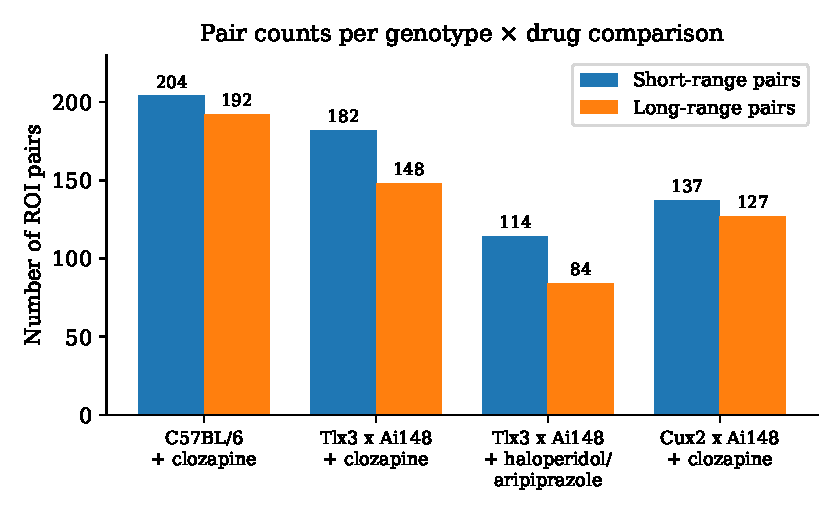
\includegraphics[width=0.78\textwidth]{figures/fig_pair_counts.pdf}
\caption{Number of short- and long-range region-of-interest (ROI) pairs entering each correlation comparison. Pairs are split at $0.9\times$ the bregma--lambda distance (${\sim}3.8$~mm). Counts reflect the pair counts reported in the experimental log for the four main comparisons across genotypes and drugs.}
\label{fig:pair_counts}
\end{figure}

% Figure 3: Mouse cohort sizes
\begin{figure}[htbp]
\centering
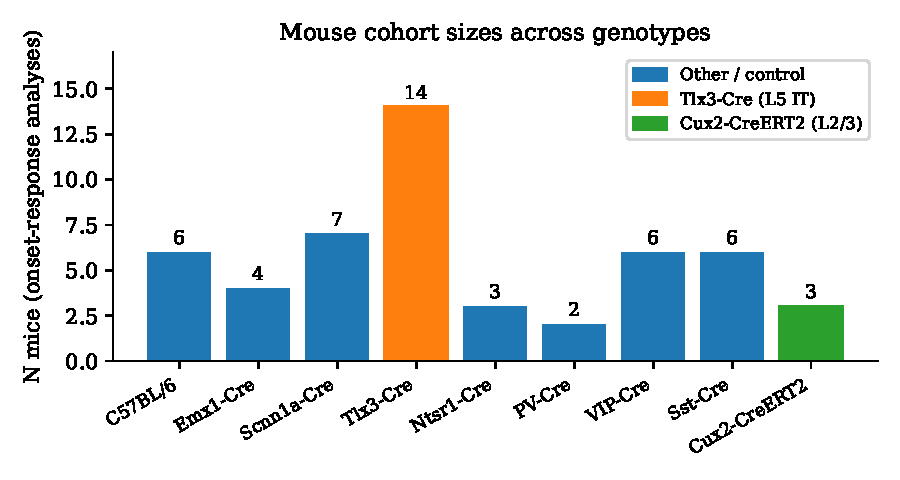
\includegraphics[width=0.90\textwidth]{figures/fig_mouse_counts.pdf}
\caption{Mouse cohort sizes across the nine genotype groups used in locomotion-onset response analyses. The Tlx3-Cre (L5 IT, highlighted orange) and Cux2-CreERT2 (L2/3, highlighted green) cohorts are the principal focus of the drug-intervention comparisons.}
\label{fig:mouse_counts}
\end{figure}

% Figure 4: p-value summary
\begin{figure}[htbp]
\centering
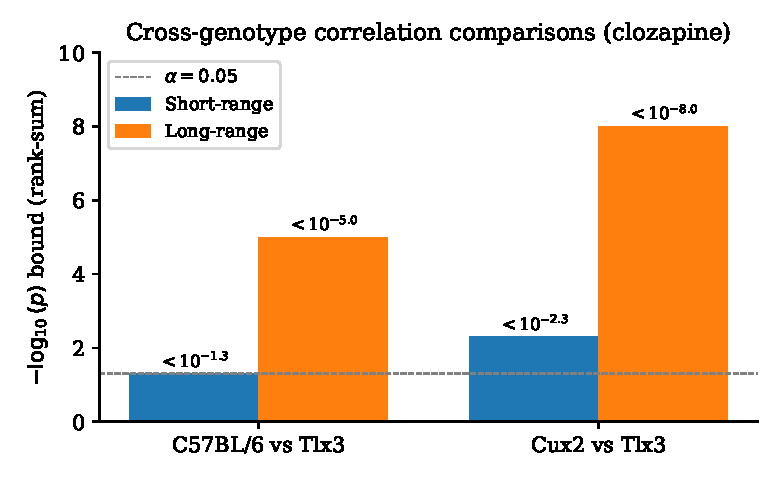
\includegraphics[width=0.70\textwidth]{figures/fig_pvalues.pdf}
\caption{Reported statistical bounds ($-\log_{10}(p)$) for cross-genotype rank-sum comparisons of correlation changes after clozapine. C57BL/6 versus Tlx3-Cre $\times$ Ai148: short-range $p<0.05$, long-range $p<10^{-5}$. Cux2-CreERT2 versus Tlx3-Cre $\times$ Ai148: short-range $p<0.005$, long-range $p<10^{-8}$. Dashed line marks $\alpha=0.05$.}
\label{fig:pvalues}
\end{figure}

% Figure 5: Session exclusion
\begin{figure}[htbp]
\centering
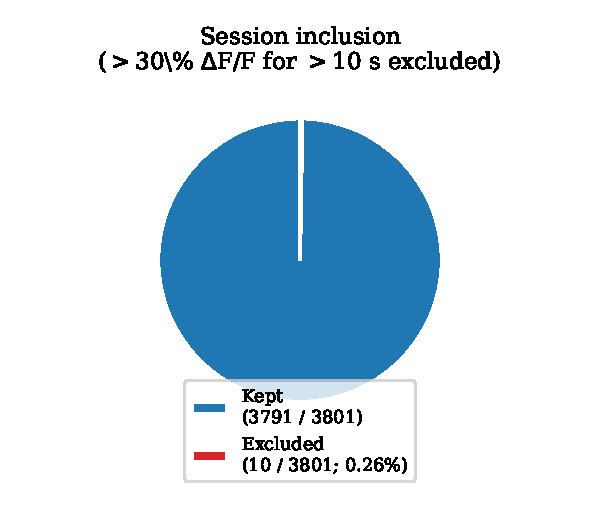
\includegraphics[width=0.55\textwidth]{figures/fig_exclusion.pdf}
\caption{Sessions were excluded if the mean activity across all 12 ROIs exceeded 30\% $\Delta F/F$ for more than 10~s. This criterion removed 10 of 3801 five-minute sessions (0.26\%).}
\label{fig:exclusion}
\end{figure}
